\chapter{Модель Изинга на динамических структурах}
\label{ch:ch3}
 
 \section{2D}
 
 \subsection{Геометрический переход}
 \label{subsection:ising_2d_struct}
 
 Для изучения перехода клубок-глобула в модели Изинга на блужданиях без  самопересечение используются геометрические характеристики: средний радиус \eqref{endtoend} и радиус вращения \eqref{gyration}. 

 \textbf{Оценка критического показателя $\nu$}.   
Критическая экспонента оценивается из степенного закона \eqref{r_scale}. Мы делаем оценку $\nu$ с помощью  линейной аппроксимации логарифмированных данных квадратов радиусов:  

  \begin{equation}
	\label{r_scale_theta_log}
 \ln \langle R_N^2 \rangle  = 2 \nu \ln N +b.  
\end{equation} 


Мы подбираем параметры $(2\nu, b)$ решая линейную регрессию в
лог-лог-пространстве, учитывая дисперсии данных. 

   \begin{figure}
	\centering
	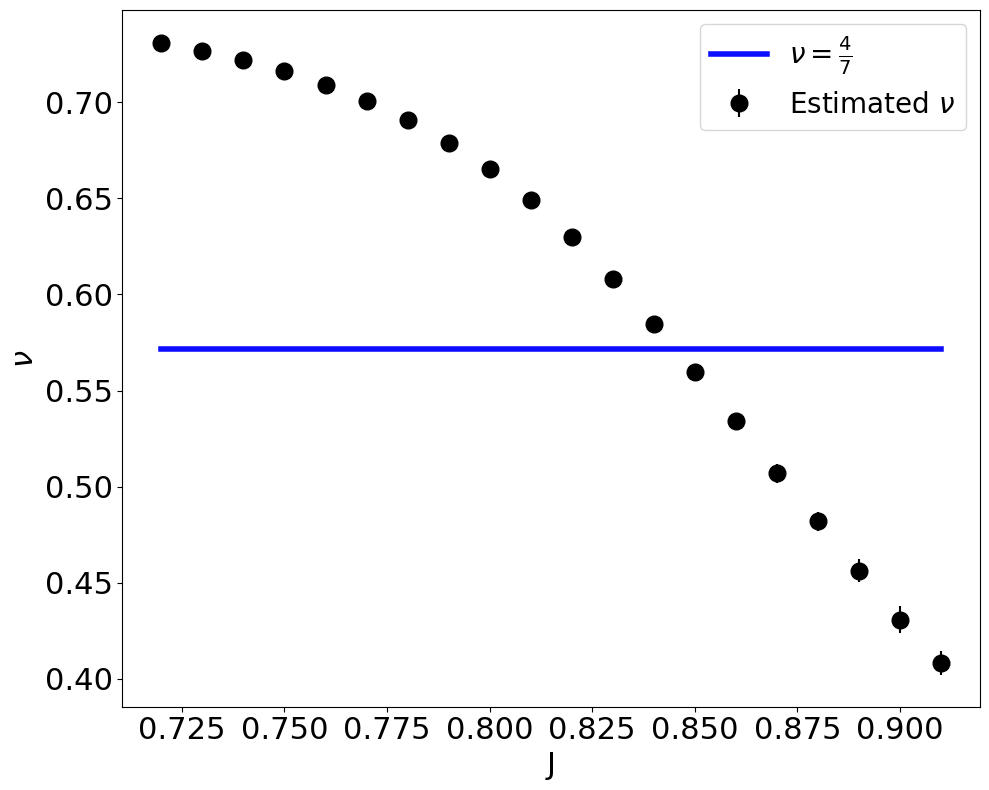
\includegraphics[scale=0.30]{images/Ising_2D_re2e_nu.png}
	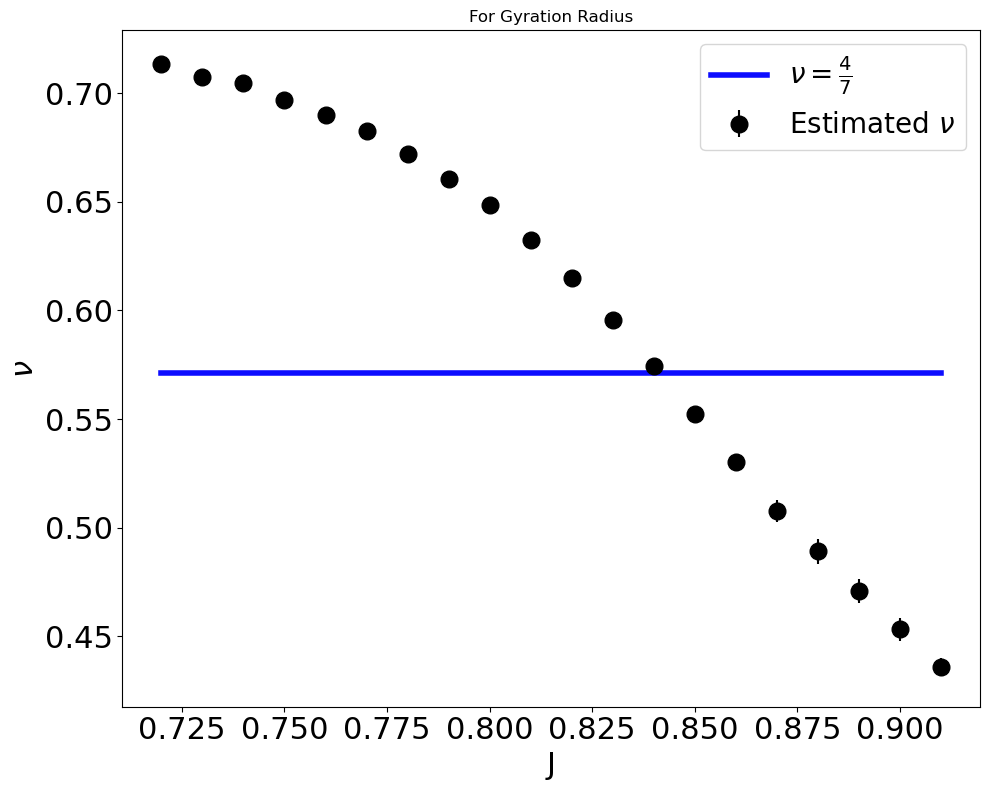
\includegraphics[scale=0.30]{images/Ising_2D_rg_nu.png}
	%\includegraphics[scale=0.18]{Images/state_example2.png}
	\caption{  Оценка критической экспоненты $\nu$ \eqref{r_scale} по численным данным среднего радиуса \eqref{endtoend} (слева) и радиуса вращения \eqref{gyration} (справа).    }
	\label{fig:ising_2d_nu_estimations}
\end{figure}

На графике  \ref{fig:ising_2d_nu_estimations} показаны полученные оценки для универсального показателя $\nu$ как функции от энергии взаимодействия $J$. Оценки, полученные по среднему радиусу и радиусу вращения, совпадают в пределах статистической погрешности 

 В области высокой температуры (малых значений $J$) показатель $\nu \rightarrow \frac{3}{4}$, что соответствует невзаимодействующему блужданию \eqref{nur}.   

В интервале $J \in [0.82; 0.85]$ показатель достигает универсального значения \eqref{nu_theta} (на графике показан синей горизонтальной линией), характерного для перехода клубок-глобула гомополимерной модели на квадратной решетке \ref{homopolymer_2d}.

В области высоких значений $J > 0.85$ показатель падает $\nu \rightarrow \frac{1}{2}$, что соответствует глобулярному режиму  \ref{globular}. Получение заниженной оценки экспоненты $\nu <  \frac{1}{2}$ объясняется конечно-размерными эффектами. 

Предварительный анализ  геометрических характеристик не противоречит предположению, что  модель Изинга на блужданиях без самопересечений проходит классический переход клубок-глобула.

\textbf{Точка структурного перехода}. 
В окрестности фазового перехода клубок-глобула средний размер полимерной цепочки (определенный через средний радиус/радиус вращения)
подчиняется следующему закону \cite{Scaling_concepts}:
   \begin{equation}
	\label{r_scale_theta}
 	\langle R_N^2 \rangle = N ^ {2 \nu _ {\Theta}} \mathcal{F} [  (J - J_{\Theta}) N ^ { 1 / \nu_c}] =  N ^ {2 \nu _ {\Theta}} \mathcal{F} [  (J - J_{\Theta}) N ^ { \phi }] , 
\end{equation} 
где  $\mathcal{F} [  (J - J_{\Theta}) N ^ { 1 / \nu_c}]$ --- универсальная  безразмерная  функция (crossover function). 
Показатель $ \phi$ ---  это «кроссоверная экспонента»,  характеризующая как быстро сужается критическая область при росте размера  цепочки. 

В критической точке $J = J_{\Theta} $ безразмерная величина 
$  \mathcal{R} (N, J)= \frac{	\langle R_N^2 \rangle }{N ^ {2 \nu _ {\Theta}}} $  не зависит от размера системы $N$. Следовательно, кривые $  \mathcal{R} (N, J)  $ в точке фазового перехода клубок-глобула пересекаются в одной точке для всех  $N$. Это позволит нам определить точку геометрического перехода. 

   \begin{figure}[ht!]%
	\centering
	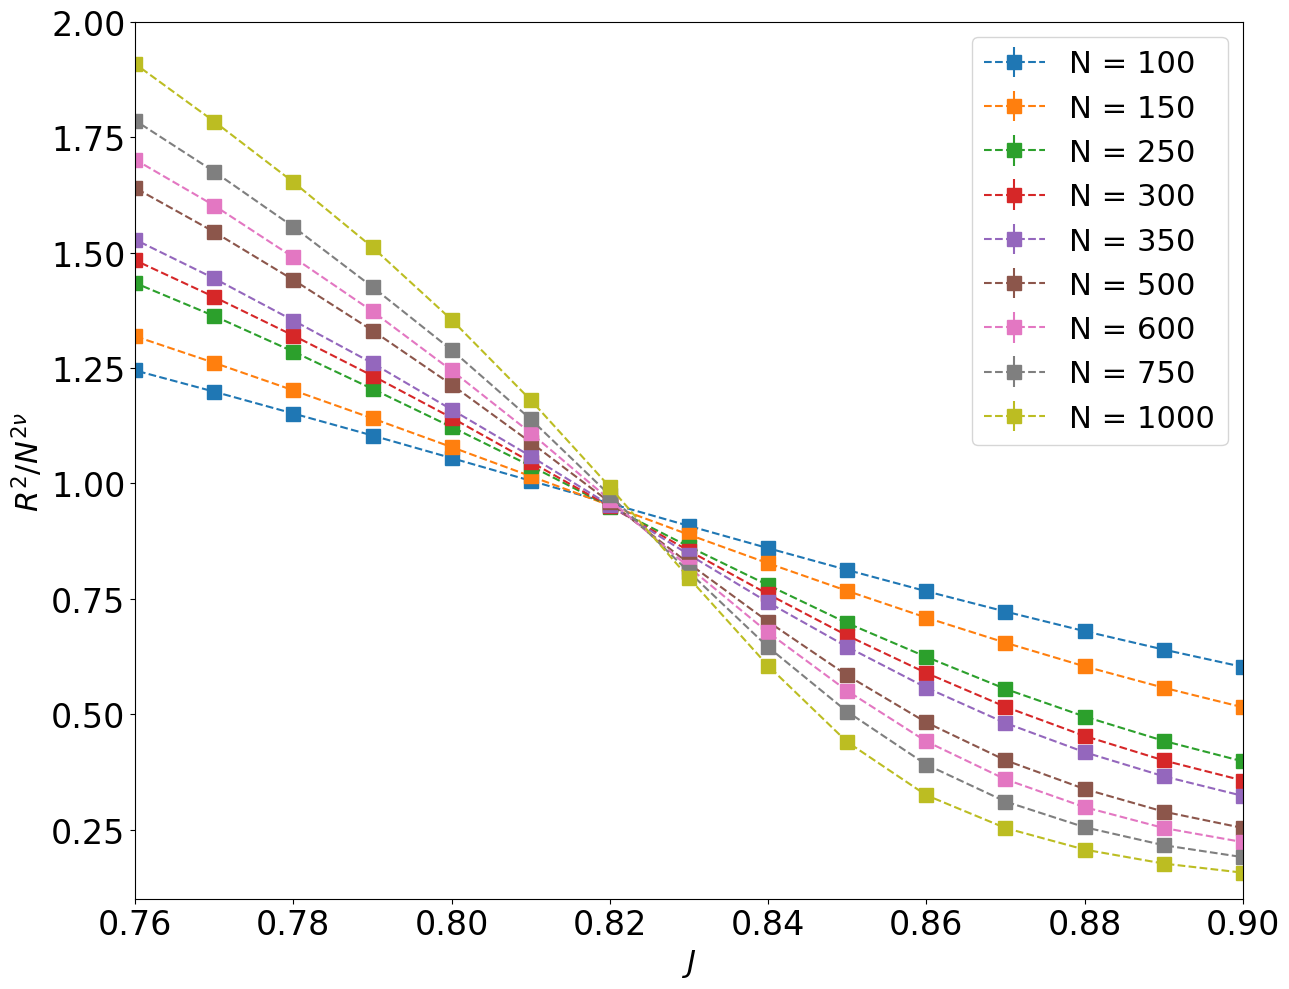
\includegraphics[scale=0.25]{images/Ising_2D_rscaling_short.png}
	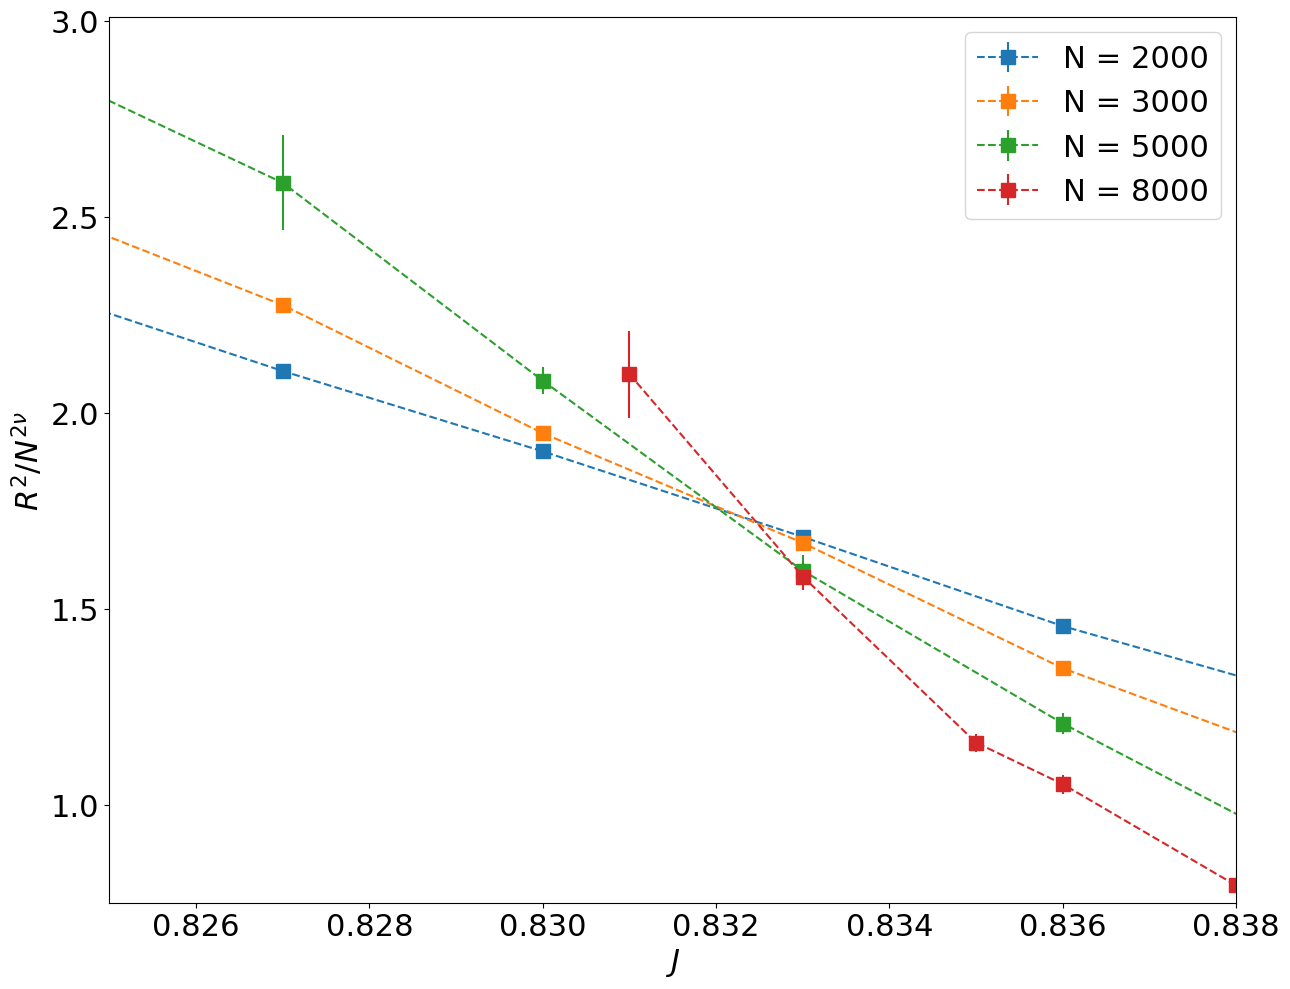
\includegraphics[scale=0.25]{images/Ising_2D_rscaling_long.png}
	\caption{ Средний радиус, отмасштабированный с фиксированным \eqref{nu_theta} как функция от $J$.      }
	\label{fig:ising_2d_rscaling}
\end{figure}
 

Для оценки точки перехода клубок-глобула мы используем данные среднего радиуса, отмасштабированного с помощью критического показателя  \eqref{nu_theta}. Отмасштабированные данные изображены на графике \ref{fig:ising_2d_rscaling}. 

Далее мы используем метод парных регрессий \ref{subsection:paired_regression} для поиска точки пересечений кривых средних радиусов и получения количественной  оценки критической точки $J_{\Theta}$. 
Мы используем $N_{fixed}=5000$ и $N_i \in [1000; 7000]$, чтобы анализировать достаточно длинные цепочки,  при этом величина погрешностей данных моделирования остаётся приемлемой. Мы получили следующую оценку:
   \begin{equation}
	\label{ising_2d_J_theta}
	J_{\Theta} \approx 0.833(1). 
\end{equation} 

Переход клубок-глобула в двумерной полимерной цепочке c Изинговым взаимодействием является непрерывным переходом второго рода. 

\begin{figure}[t]
	\centering
	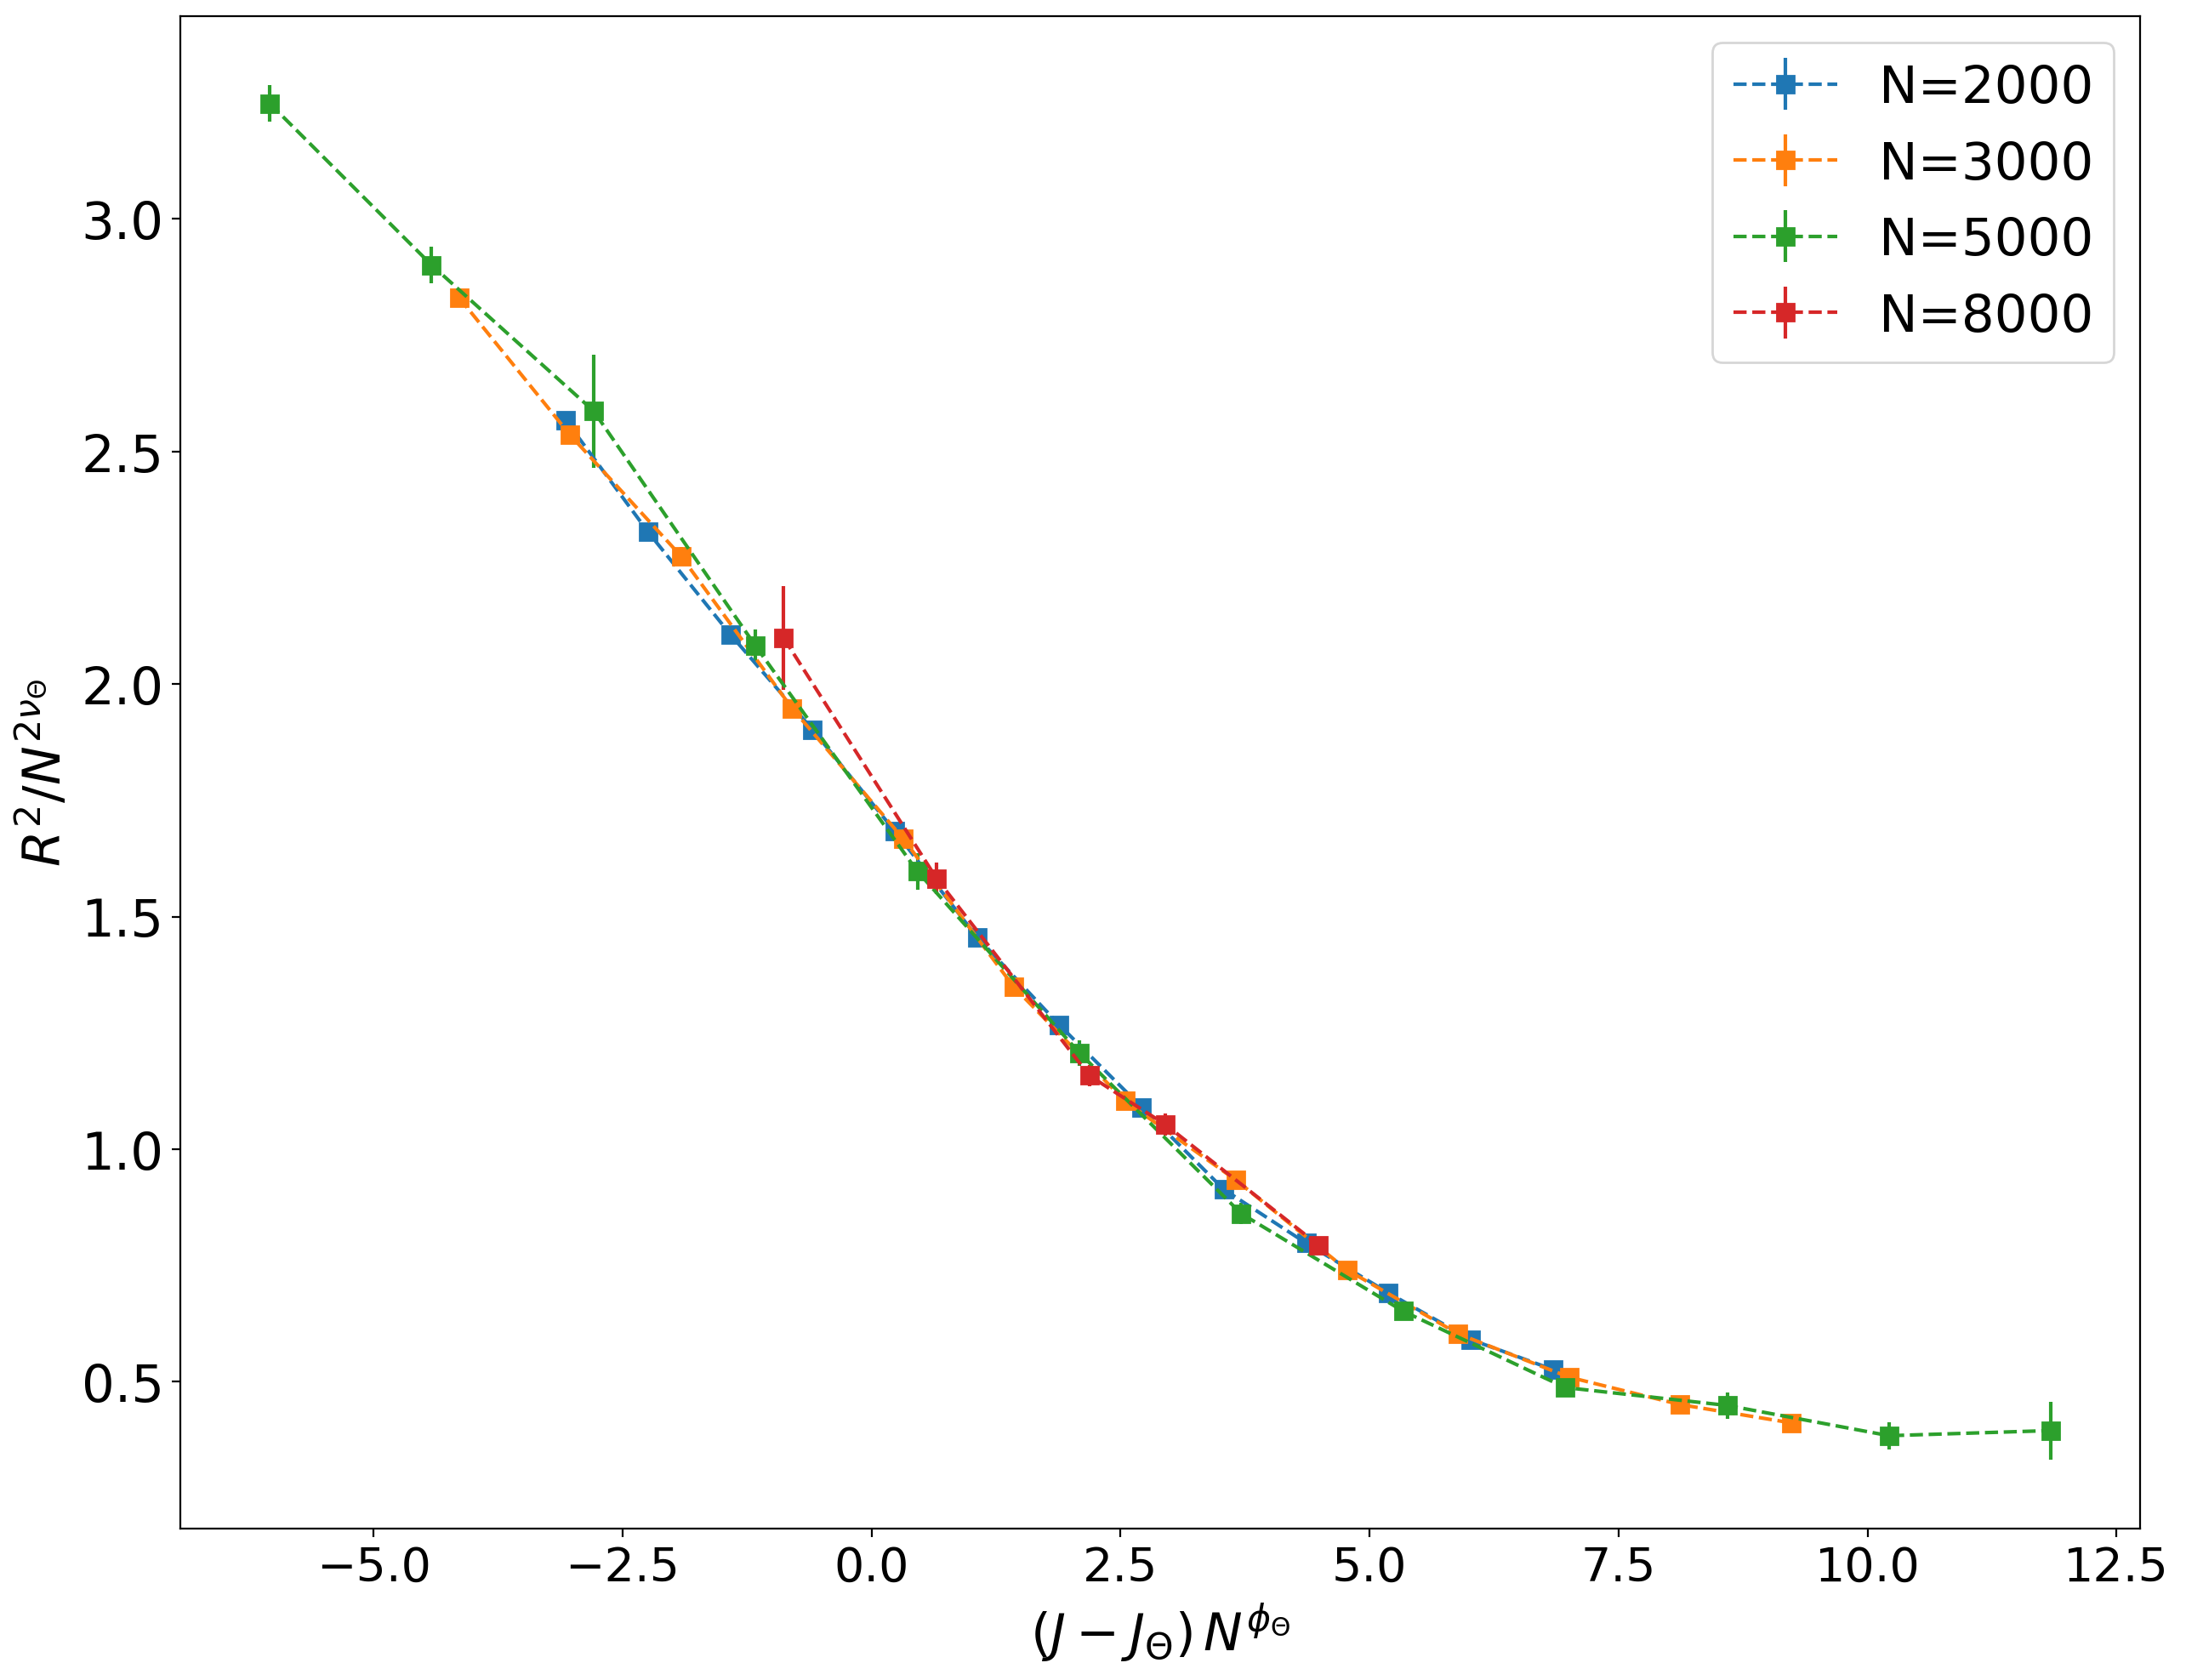
\includegraphics[scale=0.25]{images/Ising_2D_R2_collapse_auto.png}
	\caption{Коллапс кривых средних радиусов $R^2/N^{2\nu_\Theta}$ при $\nu_\Theta=4/7$ в координатах
		$X=(J-J_\Theta)N^{\phi_\Theta}$.
		Параметры коллапса: $J_\Theta=0.832150$, $\phi_\Theta^{\mathrm{eff}}=0.73913$.
		Вертикальные отрезки показывают статистические ошибки.}
	\label{fig:R2_collapse}
\end{figure}


Формула \eqref{r_scale_theta} приводит к естественным безразмерным переменным
\begin{equation}
	Y(N,J) \equiv \frac{R^2(N,J)}{N^{2\nu_\Theta}},
	\qquad
	X(N,J;J_\Theta,\phi_\Theta) \equiv (J-J_\Theta)\,N^{\phi_\Theta}.
	\label{eq:XY_defs}
\end{equation}
При корректных параметрах $(J_\Theta,\phi_\Theta)$ кривые $Y$ для разных $N$ должны накладываться на единую кривую $F(X)$.  Мы используем процедуру перебора параметров на равномерной сетке по $J_\Theta$ и $\phi_\Theta$ для получения максимально согласованного коллапса. Мы фиксируем $\nu_\Theta = 4/7$   \eqref{nu_theta}.  Для каждой длины цепочки $N$ строится
пара $(X_i^{(N)},Y_i^{(N)})$,
после чего все кривые интерполируются на общий сет $X=\{x_k\}$.
Качество коллапса оценивается взвешенной дисперсией
\begin{equation}
	\mathcal{C}(J_\Theta,\phi_\Theta)
	\;=\;
	\sum_{k}
	\sum_{N}
	w_k^{(N)}
	\Bigl[\,Y^{(N)}(x_k) - \overline{Y}(x_k)\Bigr]^2,
	\qquad
	w_k^{(N)} = \frac{1}{\bigl(\sigma^{(N)}(x_k)\bigr)^2},
	\label{eq:collapse_cost}
\end{equation}
где $\overline{Y}(x_k)$ --- взвешенное среднее по $N$ в узле $x_k$.
 
 
 На рисунке \ref{fig:R2_collapse} показаны  полученные результаты для коллапса кривых при параметрах $J_\Theta=0.832150$, $\phi_\Theta^{\mathrm{eff}}=0.73913$. 
 Кривые для разных $N$ практически накладываются друг на друга. Значение $J_\Theta$, полученная поиском максимально согласованного коллапса,  согласуется с оценками по пересечениям \eqref{ising_2d_J_theta} при фиксированном $\nu_\Theta$. 
 
 
 Отметим, что полученное значение $\phi_\Theta^{\mathrm{eff}}\approx 0.74$ заметно выше теоретического трикритического значения $3/7\simeq 0.4286$. Однако, завышенные оценки при численном моделировании были также получены и для классического гомополимера $\phi_\Theta^{\mathrm{eff}}\approx 0.48$  \cite{Caracciolo_2011}, хотя и в меньшей степени.  

 \subsection{Магнитный переход}
 
 \textbf{Намагниченность}.   
 Численные данные второго момента намагниченности в зависимости от константы $J$ представлены на графике \ref{fig:ising_2d_mags}. При малых значениях $J$ система находится в парамагнитном состоянии (также предел $J->0$ соответствует модели БСП без взаимодействия  \ref{homopolymer_2d} ). 
 
 В интервале $J\in  [0.82;0.85] $ наблюдается подъём кривых второго момента намагниченности --- в этой области происходит фазовый переход из неупорядоченного (парамагнитного) режима в упорядоченный (ферромагнитный). С увеличением $N$ подъем становится более резким, а точка перегиба сосредоточивается около  значения $J\approx 83.5$. 
 
   \begin{figure}[ht!]
 	\centering
 	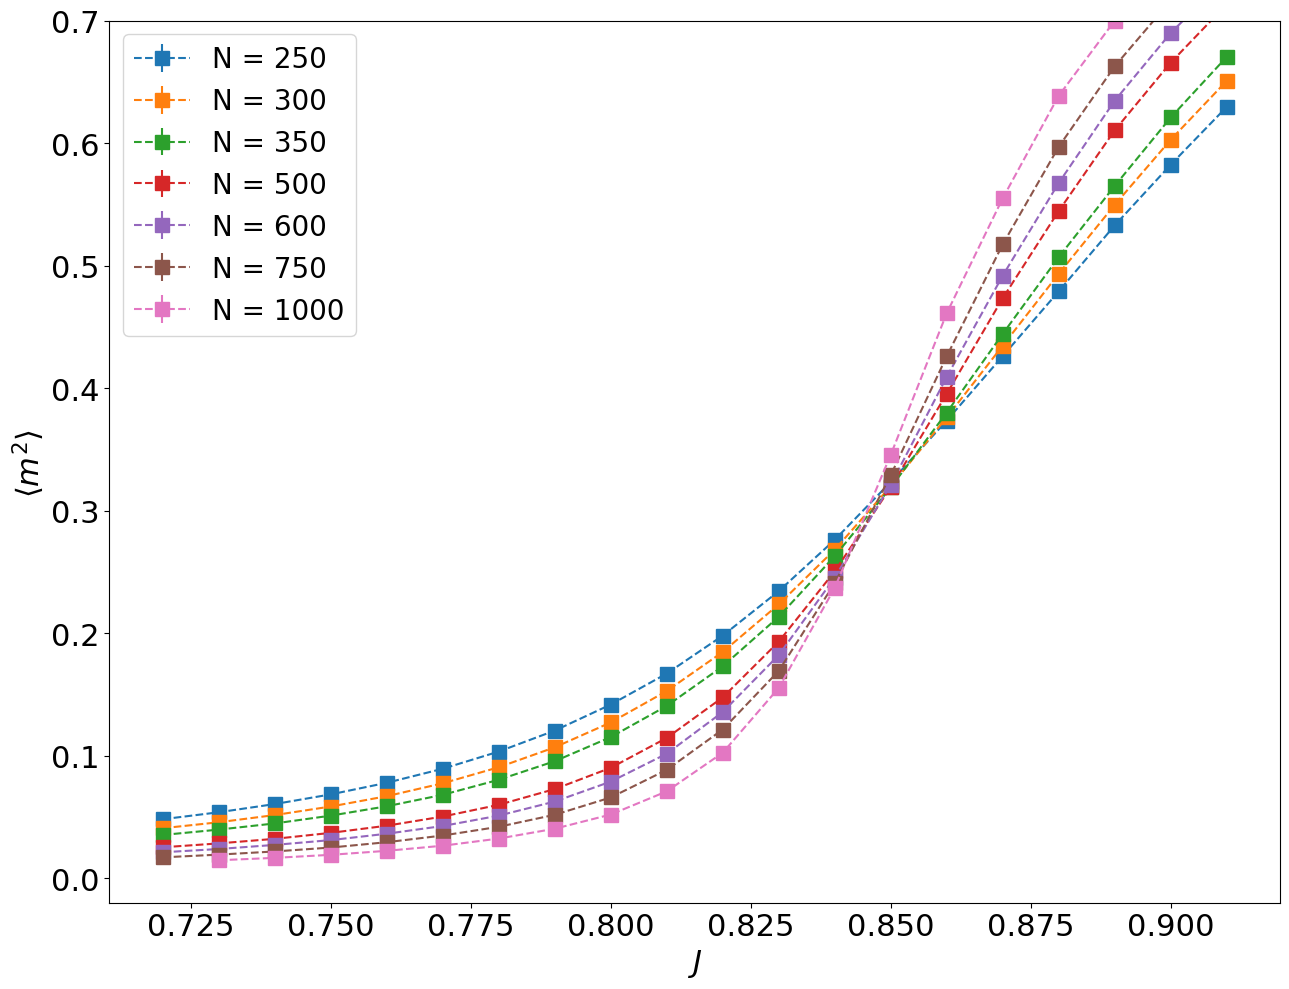
\includegraphics[scale=0.25]{images/Ising_2D_rg2_m2_short.png}
 	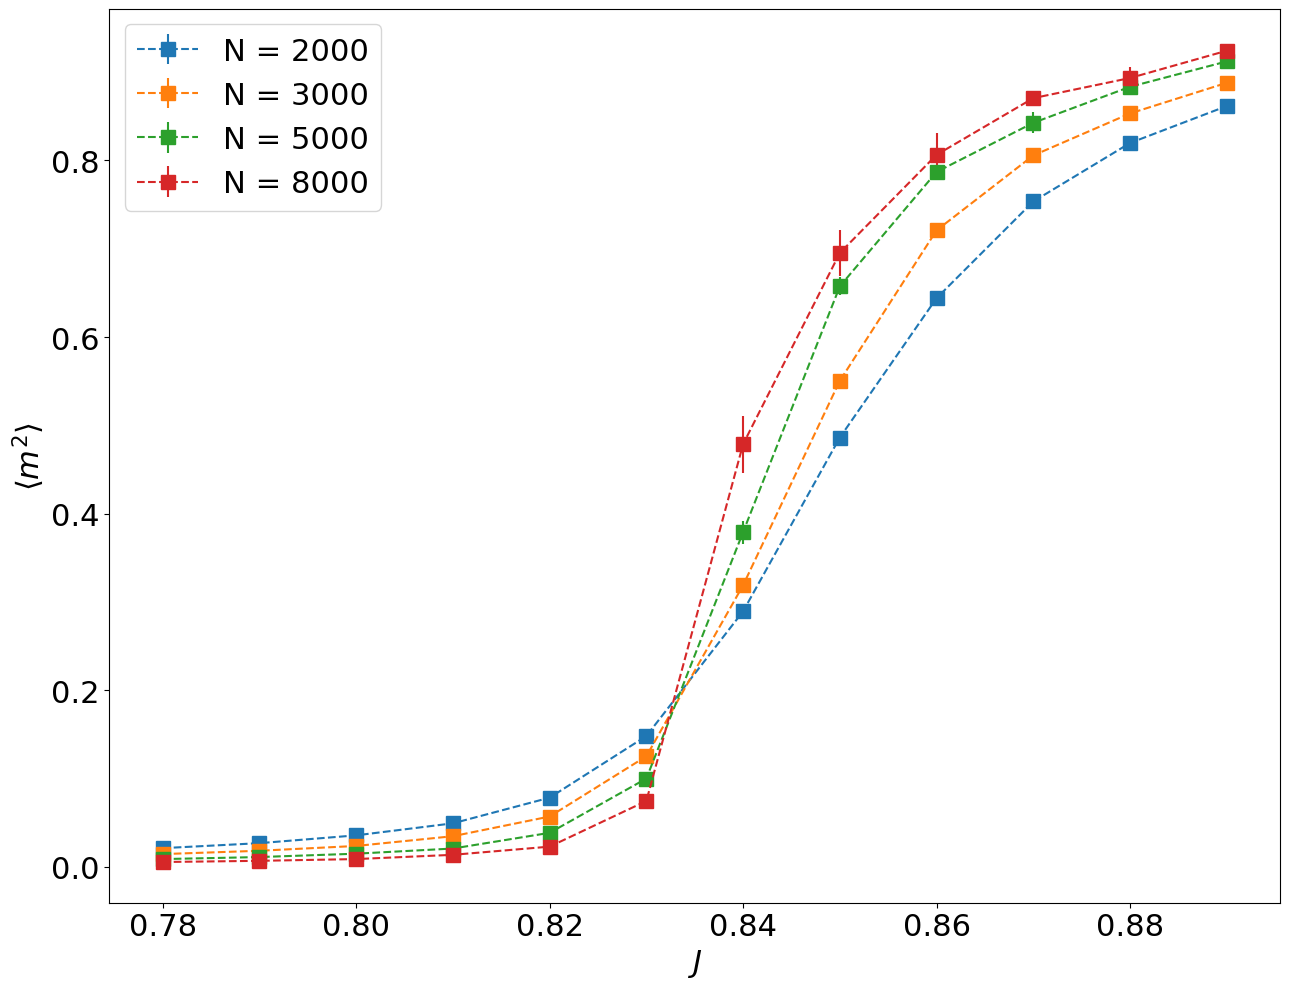
\includegraphics[scale=0.25]{images/Ising_2D_rg2_m2_long.png}
 	%\includegraphics[scale=0.18]{Images/state_example2.png}
 	\caption{ Второй момент намагниченности    \eqref{ising_mean_magnetization} как функции от  $J$.     }
 	\label{fig:ising_2d_mags}
 \end{figure}
  
  
   \textbf{Энергия}.  
  
      \begin{figure}
   	\centering
   	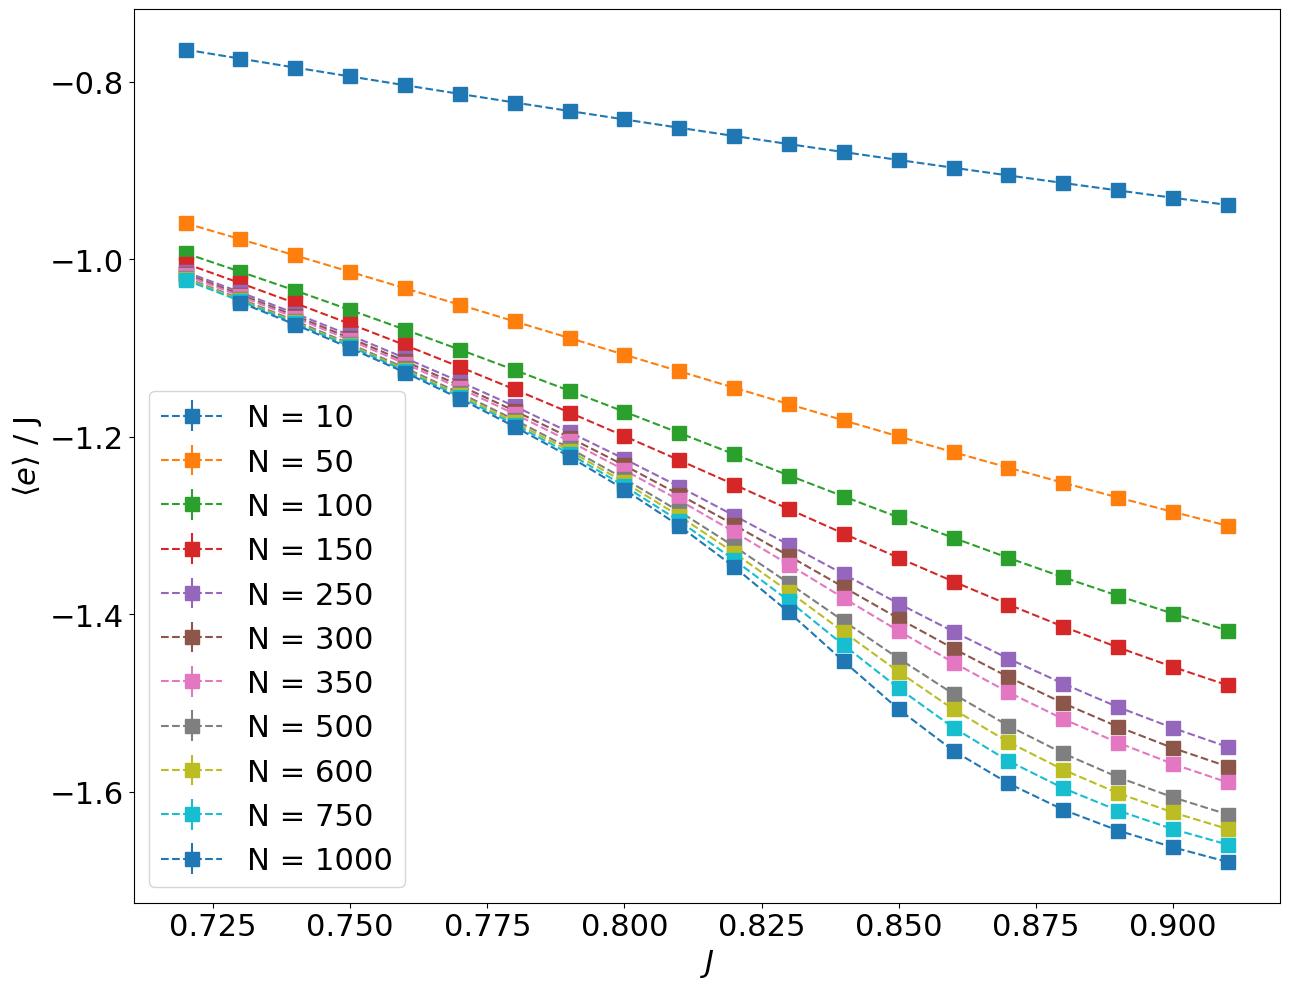
\includegraphics[scale=0.25]{images/Ising_2D_rg2_e1_short.png}
   	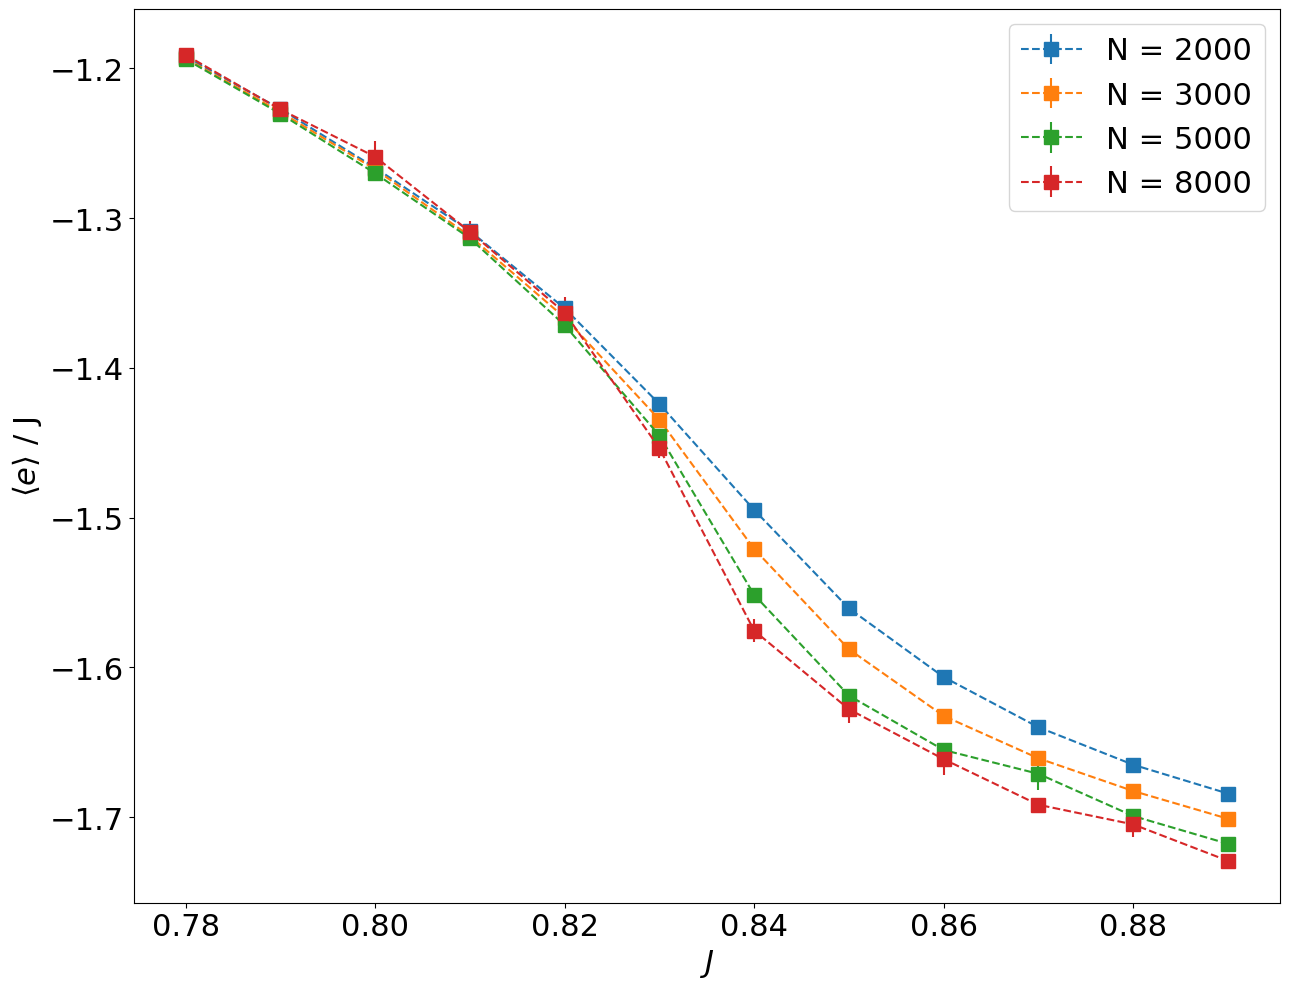
\includegraphics[scale=0.25]{images/Ising_2D_rg2_e1_long.png}
   	%\includegraphics[scale=0.18]{Images/state_example2.png}
   	\caption{ Первый момент энергии на спин как функции от  $J$.     }
   	\label{fig:ising_2d_energy}
   \end{figure} 
     
     На рисунке \ref{fig:ising_2d_energy} показано, как средняя энергия на спин  монотонно убывает c ростом энергии взаимодействия $J$. 
     Так, энергетические данные подтверждают магнитный критический переход, согласуясь с поведением второго момента намагниченности.
        
        
        
    \textbf{Теплоемкость}. 
     Для продолжения анализа фазового магнитного перехода рассмотрим еще одну физическую величину --- теплоемкость: 
    \begin{equation}
    	\label{eq:capacity_heat}
    	C_N(J) \;=\; \frac{\partial \langle E\rangle}{\partial J}
    	\;=\; \mathrm{Var}(E) \equiv \langle E^2\rangle - \langle E\rangle^2,
    \end{equation}
    
    Удобно работать с удельной величиной $c_N(J)=C_N(J)/N$. При переходе первого рода пик удельной теплоемкости машстабируется следующим образом: 
    \(
    c_N^{\max}\sim N^{\alpha} \sim N. 
        \)   
    При  непрерывном переходе:
    \(
    c_N^{\max}
    \)
    растёт сублинейно (логарифмически или степенной  показатель $\alpha<1$) \cite{PhysRevB.34.1841} \cite{Landau_Binder_2021}. 
    
        \begin{figure}
    	\centering
    	\includegraphics[scale=0.25]{images/ising_heat_c_vs_J.png}
    	\includegraphics[scale=0.25]{images/ising_heat_cmax_scaling.png}
    	\caption{ Численные данные для удельной теплоемкости \eqref{eq:capacity_heat}. На левом графике  в качестве ошибок показана верхняя граница. Оценки пиков теплоемкости показаны черными точками для каждой длины цепочки $N$. }
    	\label{fig:C_vs_J_short}
    \end{figure} 
        
        
      Полученные компьютерным моделированием кривые удельной теплоемкости \eqref{eq:capacity_heat}  показаны на графике  \ref{fig:C_vs_J_short}. 
      Максимум удельной теплоемкости монотонно растёт с $N$, но его рост 
      существенно медленнее линейного (оценка параметра  $\alpha \approx 0.36 \pm 0.05$). Такое поведение согласуется с непрерывным переходом. 
        
        
 \textbf{Кумулянты Биндера для намагниченности}.  Для изучения фазового магнитного перехода рассмотрим кумулянт Биндера четвертого порядка для намагниченности  \eqref{binder_cumulant}.  
 
       \begin{figure}
 	\centering
 	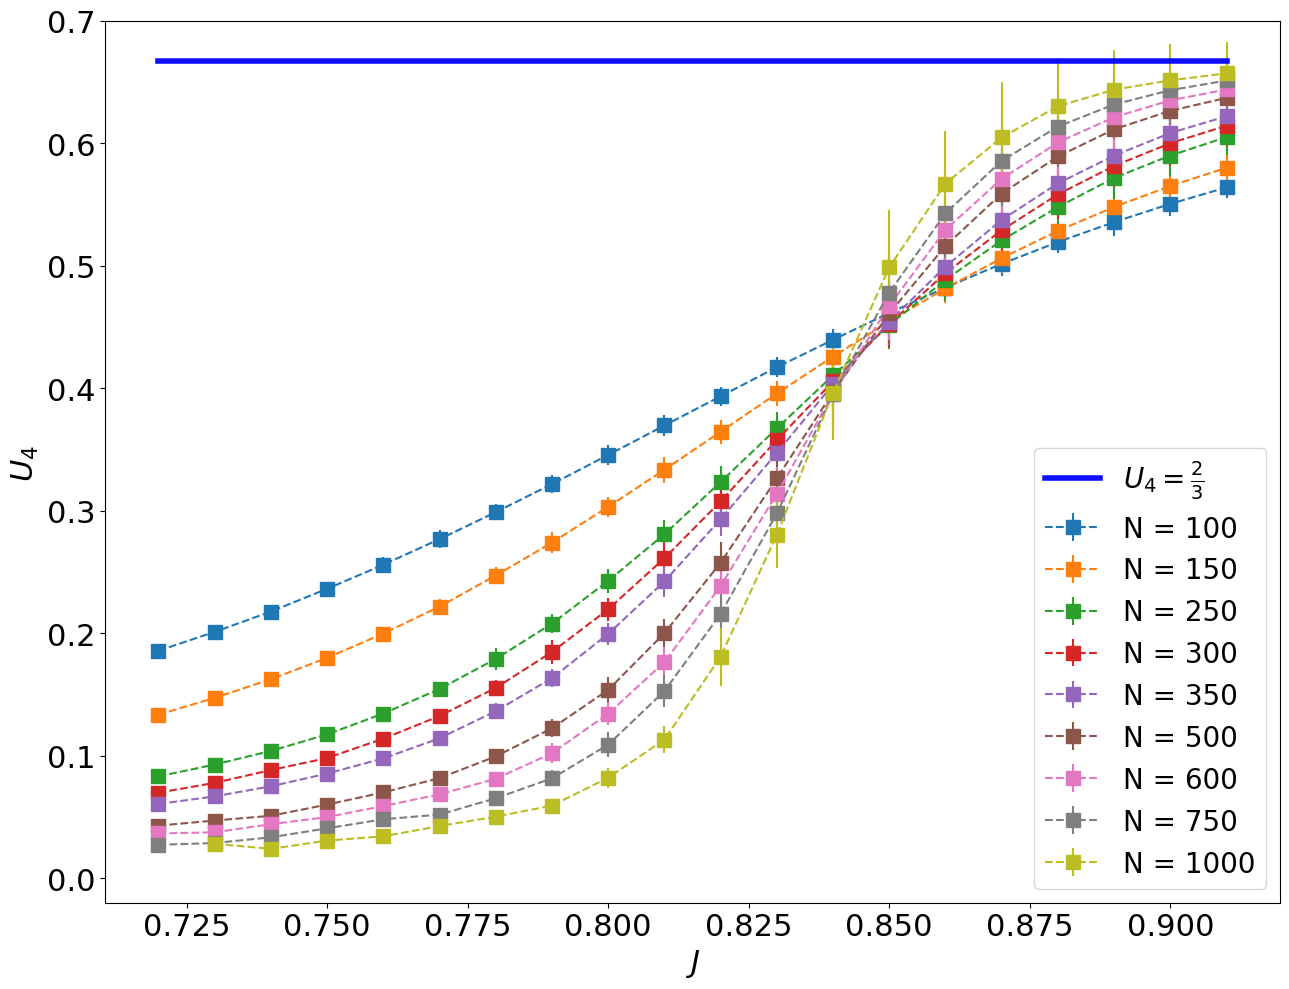
\includegraphics[scale=0.25]{images/Ising_2D_U4_short.png}
 	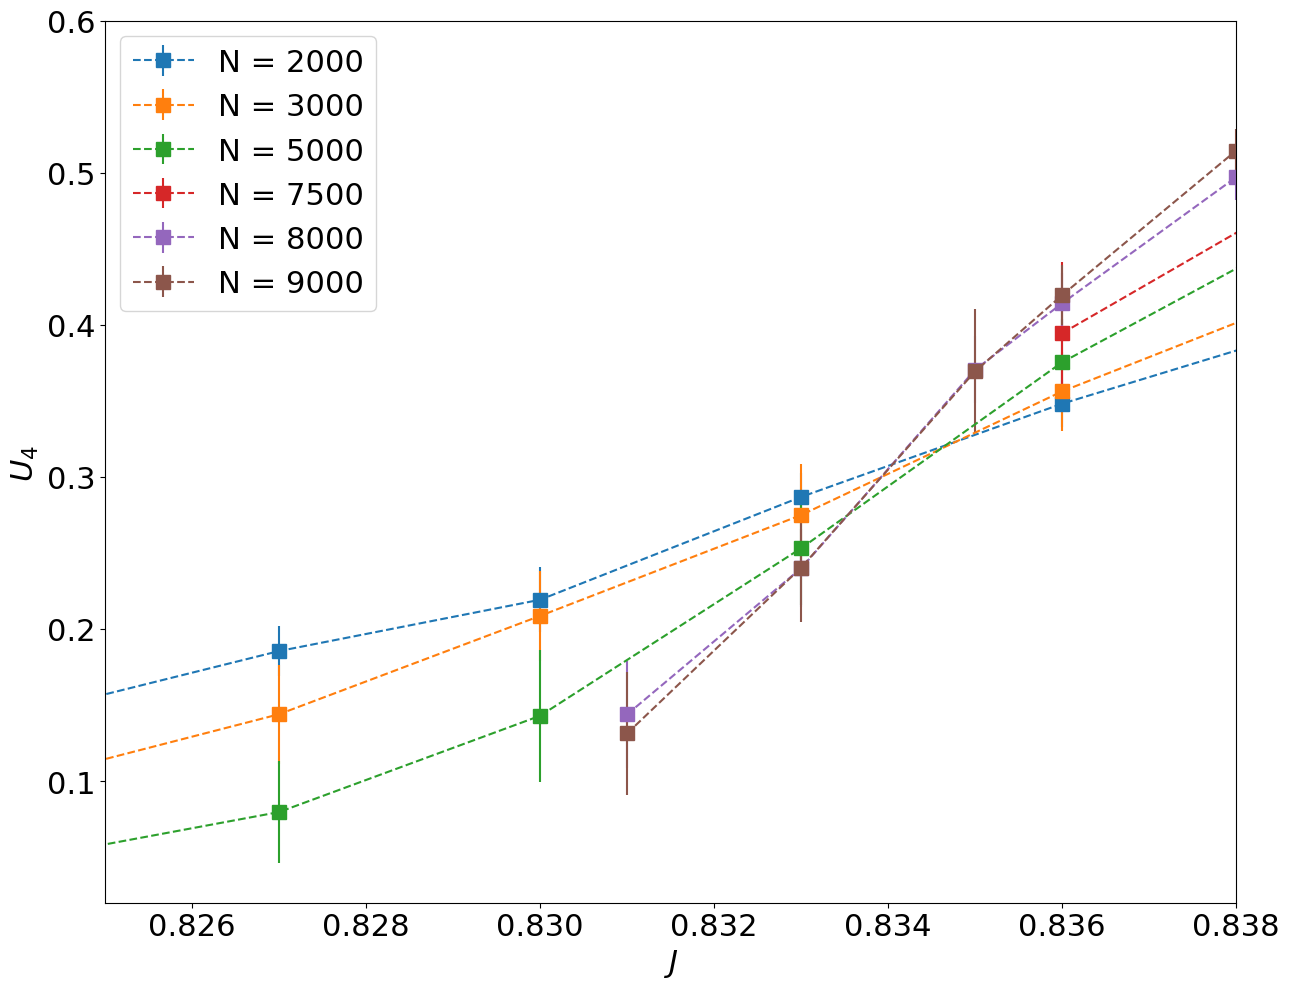
\includegraphics[scale=0.25]{images/Ising_2D_U4_long.png}
 	%\includegraphics[scale=0.18]{Images/state_example2.png}
 	\caption{ Кумулянты Биндера \eqref{binder_cumulant}  как функции от  $J$.     }
 	\label{fig:ising_2d_U4}
 \end{figure} 
 
 На графике  \ref{fig:ising_2d_U4}  показаны полученные кривые кумулянтов. В интервале $J \in [0.83; 0.85]$ кривые кумулянтов для разных длин $N$ пересекаются. Такое поведение согласуется с картиной
 непрерывного (второго рода) магнитного перехода. 
  
  Воспользуемся методом парных регрессий \ref{subsection:paired_regression} для оценки критической точки фазового перехода. Аналогично анализу структурного перехода \ref{subsection:ising_2d_struct}, возьмем $N_{fixed}=5000$ и $N_i \in [1000; 9000]$. Получим следующие оценки для критических значений: 
  
   \begin{equation}
  	\label{Ising_2d_U4_cr} 
  	 U^{cr}_4	=  0.308,
  \end{equation}  
 
  \begin{equation}
  	\label{Ising_2d_J_cr} 
  J_{cr}	= 0.8340(5). 
  \end{equation}  
   
   
     
 \subsection{Распределения энергии.}
\begin{figure}[ht!]
 	\centering
 	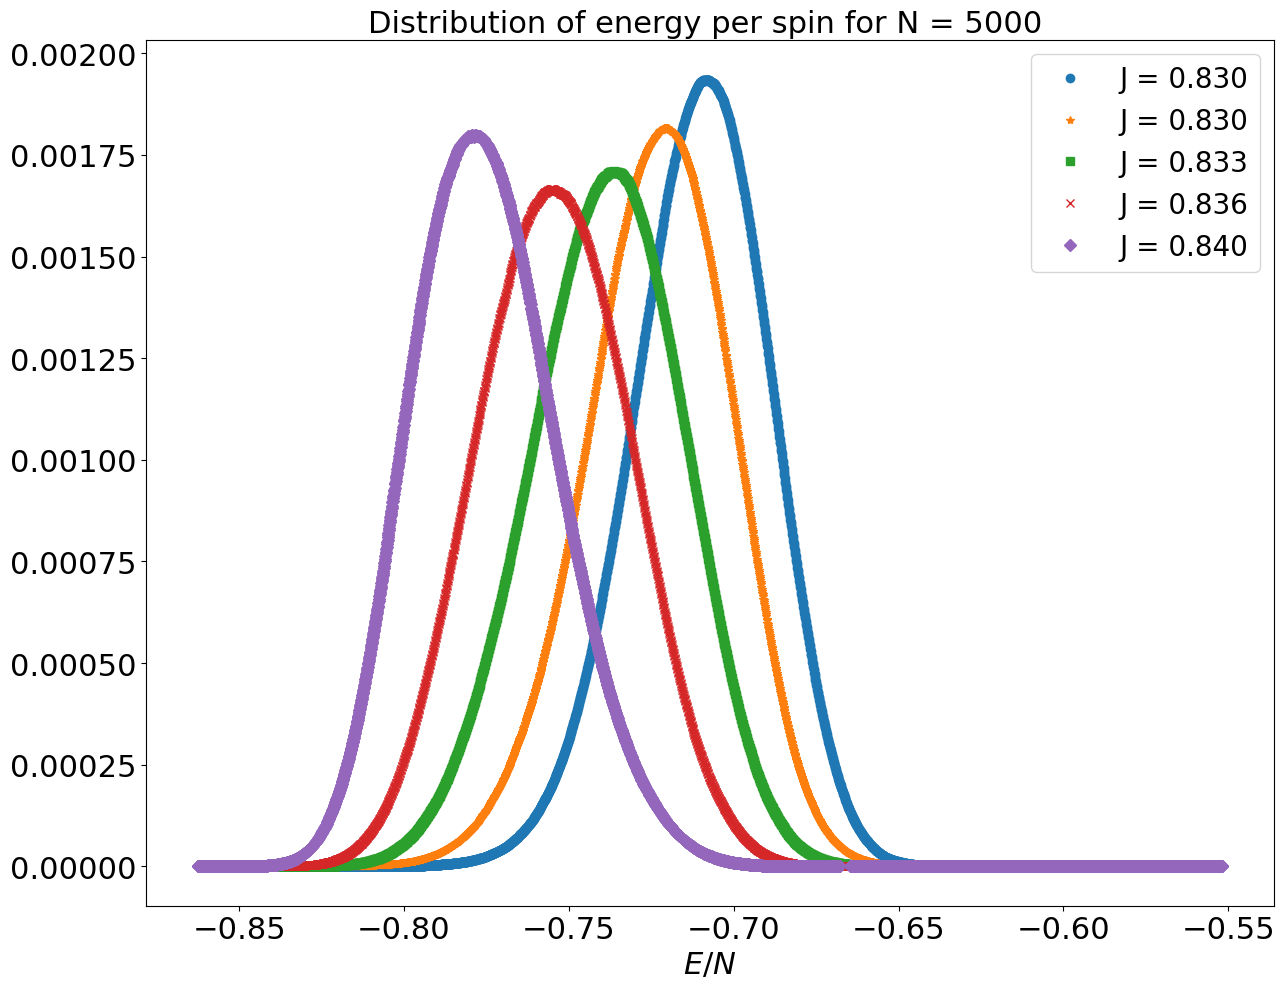
\includegraphics[scale=0.25]{images/Ising_distrenergy_5000.png}
 	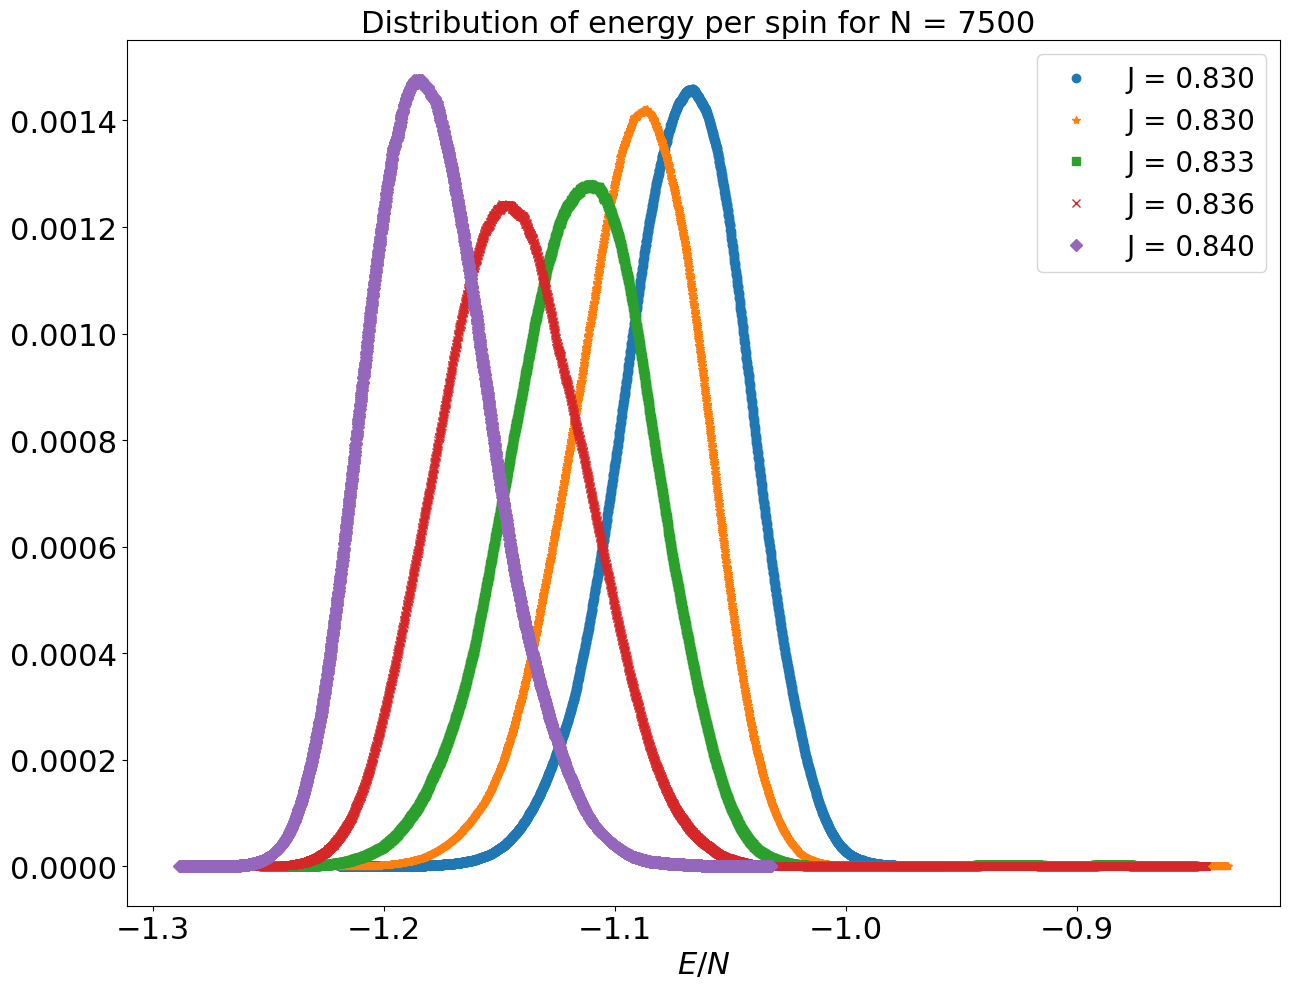
\includegraphics[scale=0.25]{images/Ising_distrenergy_7500.png}
 	\caption{  Распределения энергии на спин для цепочек длины  $N=5000$ (слева)  и  $N=7500$  (справа).}
 	\label{fig:ising_2d_distr_E}
 \end{figure} 
  Для дальнейшего изучения характера фазового перехода мы рассмотрим распределения энергии на спин. На графике  \ref{fig:ising_2d_distr_E}  изображены распределения энергии на спин для цепочек длины  $N=5000$ (слева)  и  $N=7500$  (справа) в интервале, включающем полученные оценки критических точек \eqref{Ising_2d_J_cr}  и  \eqref{ising_2d_J_theta}. Полученные формы распределений являются одномодальными, что соответствует непрерывному фазовому переходу. 
 
 
  \subsection{Вывод} 

 Оценки для магнитного перехода \eqref{Ising_2d_J_cr}   и перехода клубок-глобула \eqref{ising_2d_J_theta} согласуются в пределах погрешности.  
 
 Анализ геометрических характеристик показал, что структурный переход в двумерной полимерной цепочке c Изинговым взаимодействием является непрерывным переходом. Наши вычислительные результаты показывают, что при конформационном переходе критический показатель  $\nu=4/7$  наследуется от тета-полимера \eqref{nu_theta}. 
 
 Анализ термодинамических характеристик показал, что магнитный переход в системе является переходом второго рода. 
 